%!TEX root = thesis.tex
\chapter{2-D Imaginary Time Evolving Block Decimation}
\label{chapter:2ditebd}

In one-dimensional many-body systems, the performance of one-dimension imaginary time evolving block decimation (1D-iTEBD) is very well, especially its high efficiency. Naturally, people want to extend the framework to study the two-dimensional systems. However, through many experiments we notice that the accuracy in 2-D is less than 1-D. In order to resolve that the obstacle, optimizations of 2-D algorithms became an essential part in condense matter physics. 

In the sections \ref{ite} and \ref{itebd}, we briefly review the idea of imaginary time evolution (TEBD) \cite{vidal_efficient_2003} \cite{vidal_efficient_2004} and explain how to extend it to simulate an infinite two-dimensional system (2D-iTEBD)\cite{li_efficient_2012}. However, the method recorded in ref.\cite{li_efficient_2012} is unstable because it need multiply too many pseudo-inverse matrices during updating the wave functions. Hence, In the sections \ref{2dhastin} and \ref{2dopt} we record more advance discussions about optimizing 2D-iTEBD, such as the method developed by Hastings \cite{}, combined with QR decomposition, and so on. In the final section \ref{Comparison}, we utilize 2D-iTEBD to simulate the toy models, Heisenberg and transverse Ising, on two-dimensional square lattice and compare the features among 2D-TEBD algorithms which are implemented by different way. Notice that in this chapter we just focus on obtaining good projected entangled pair states \cite{} by 2D-iTEBD. The optimization of measurement (accuracy) will be discussed in chapters \ref{chapter:ctm}.


\section{Imaginary Time Evolution}
\label{ite}
In the section, we apply the conclusion of the theory of imaginary time evolution and matrix product states (MPS) \cite{} to explain the fundamental concept of TEBD-like algorithms. Theoretically, if existing the imaginary time evolution operator $e^{-\tau H}$, where $H$ is the Hamiltonian of a specified model, we could project any initial random states to the ground state,
\begin{align}
	\label{mapgroud}
	\Ket{\psi_0} = \frac{e^{-\tau H} \Ket{\Psi}}{\parallel e^{-\tau H} \Ket{\Psi}\parallel}
\end{align}
However, according to eq.\ref{wavefunc}, we notice that the number of coefficients in an origin evolution operator $e^{-\tau H}$ is proportional to $d^N \times d^N$. In other words, it is impossible to update entire system directly. Therefor, in 1D quantum many-body systems we apply MPS structure to restrict the exponential increment of dimension. Base on the theory of the MPS, the wave function composed by pure states can be decompose to many unit cells by \textit{sigular value decomopostion} and \textit{Schmidt decomposition}. To explain the MPS structure more explicitly, we begin from splitting the wave function $\Ket{\Psi_N}$ [Fig. \ref{fig225}(a)] between $n$ and $n+1$ sites with Schmidt decomposition, 
\begin{align}
	\label{schmitwave}
	\Ket{\Psi_{N}} = \sum_{\alpha_n} \lambda_{\alpha_n} \Ket{\psi_{\alpha_n}^{[1\dots n]}} \Ket{\psi_{\alpha_n}^{[n+1\dots N]}}
\end{align}
where $\lambda_{\alpha_n} > 0$ and $\sum\limits_{\alpha+n}{\lambda_{\alpha_n}^2 = 1}$. To obtain the one site wave function $\Ket{\psi_{\alpha_n}^{[n+1]}}$, we perform Schmidt decomposition on $\Ket{\psi_{\alpha_n}^{[n+1\dots N]}}$ between the $n+1$ and $n+2$ sites,
\begin{align}
	\Ket{\psi_{\alpha_n}^{[n+1\dots N]}} = \sum_{\alpha_{n+1}} \lambda_{\alpha_{n+1}} \Ket{\psi_{\alpha_{n+1}}^{[n+1]}} \Ket{\psi_{\alpha_{n+2}}^{[n+2\dots N]}}
\end{align}
then span $\Ket{\psi_{\alpha_{n+1}}^{[n+1]}}$ by the spin basis $i_{n+1}$,
\begin{align}
	\Ket{\psi_{\alpha_{n+1}}^{[n+1]}} = \sum_{i_{n+1}}{\Gamma^{[n+1] i_{n+1}}_{\alpha_n \alpha_{n+1}} \Ket{i_{n+1}}}
\end{align}
and the Eq. \ref{schmitwave} can be re-written as, 
\begin{align}
	\Ket{\Psi_{N}} = \sum_{\alpha_n,\alpha_{n+1}}\sum_{i_{n+1}}{\lambda_{\alpha_n} \Gamma^{[n+1] i_{n+1}}_{\alpha_n \alpha_{n+1}} \lambda_{\alpha_{n+1}l} \Ket{\psi_{\alpha_n}^{[1\dots n]}} \Ket{i_{n+1}} \Ket{\psi_{\alpha_{n+2}}^{[n+2\dots N]}} }
\end{align}
In the end, we can perform the same process site-by-site in the entire system and obtain the MPS structure,
\begin{align}
	\Ket{\Psi_N} = \sum_{\alpha_1,\dots ,\alpha_N}\sum_{i_1,\dots ,i_N}{ \Gamma^{[1] i_{1}}_{\alpha_1} \lambda_{\alpha_1} \Gamma^{[2] i_{2}}_{\alpha_1 \alpha_{2}} \lambda_{\alpha_2} \dots  \lambda_{\alpha_{N-2}} \Gamma^{[N-1] i_{N-1}}_{\alpha_{N-2} \alpha_{N-1}} \lambda_{\alpha_{N-1}} \Gamma^{[N] i_{N}}_{\alpha_{N}} \Ket{i_1 i_2 \dots i_N}}
\end{align}
and the tensor network representation is shown as Fig. \ref{fig311}, 
\begin{figure}[ht]
	\centering
	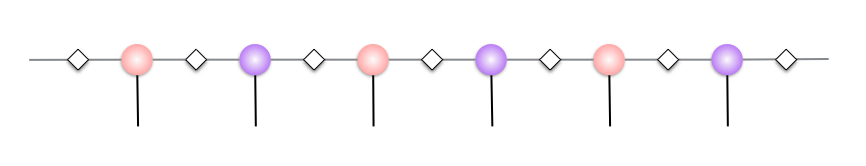
\includegraphics[width=0.90\textwidth]{figures/fig311.png}
	\caption[The tensor network representation of matrix product states]{The tensor network representation of matrix product states.}
	\label{fig311}
\end{figure}

Now that we try to expand it to a infinite chain \cite{}. Since the translation invariance, the wave function $\Ket{\Psi_{N=\infty}}$ can be represent as $n$-site translational symmetric states, which means that $\Gamma^{[i]}$ and $\lambda^{[i_{i}]}$ are independent of $\Gamma^{[i+n]}$ and $\lambda^{[i+n]}$. For instance, the tensor diagram can be drawn as Fig.\ref{fig312}, when $n=2$, which means that the wave function of a infinite chain can be recognized as a composite of matrix product states $\lambda^{[A]}\Gamma^{[A]}$ (red nodes) and $\lambda^{[B]}\Gamma^{[B]}$ (purple nodes).

\begin{figure}[ht]
	\centering
	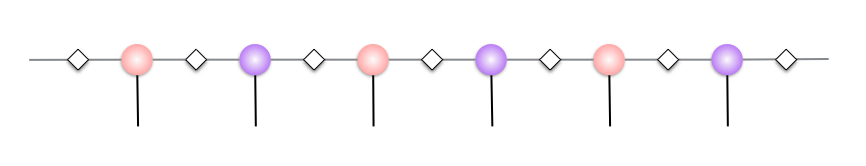
\includegraphics[width=0.90\textwidth]{figures/fig311.png}
	\caption[The tensor network representation of matrix product states]{The tensor network representation of matrix product states.}
	\label{fig312}
\end{figure}

Next, in order to update the two states in the unit cell, we utilize the \textit{Suzuki Trotter decomposition} to approximate the entire evolution operator with $2$-sites operators, \textit{The first-order Suzuk-Trotter decompostio} of operator $e^{\delta (A+B)}$ is,
\begin{align}
	\label{STd}
	e^{\delta A + B} = e^{\delta A}e^{\delta B} + O(\delta^2)
\end{align}
where $A$ and $B$ are two non-commutative operators.Therefor, we can approximate the entire evolution operator by grouping the two site operator $H_{AB}$ and $H_{BA}$,
\begin{align}
	\label{evoopt}
	e^{-\tau H} = \left(e^{-\delta H}\right)^{\frac{\tau}{\delta}} \approx \left(\prod e^{\delta H_{AB}} \right)\left( \prod e^{\delta H_{BA}}\right)
\end{align}
Therefor, we can obtain the evolution operator $e^{H_{AB}}$ and $e^{H_{BA}}$ straightly after solving two site $H_{AB}$ and $H_{BA}$.
So far, we have obtained the infinite MPS composed by 2-site unit cells and the 2-site evolution operators $e^{-\tau H_{AB}}$ and $e^{-\tau H_{BA}}$. Hence, the tensor network representation of Eq. \ref{mapgroud} can be drawn as Fig. \ref{fig313}, which means that the ground state $\Ket{\psi_0}$ can be regard as contracting all the tensors in the diagram. So the next problem: How can we contract them and preserve the structure like Fig{\ref{fig311}}?

\begin{figure}[ht]
	\centering
	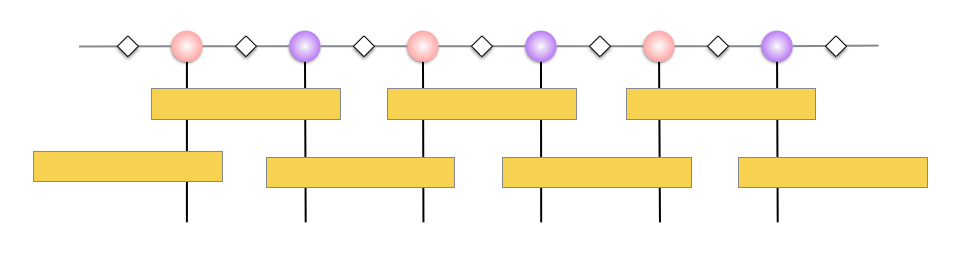
\includegraphics[width=0.90\textwidth]{figures/fig312.png}
	\caption[The picture of the main idea of itebd.]{The red and blue tensor denotes on \textit{odd} and \textit{even} sites. The yellow one are time evolution operators $e^{-\tau H_{k,k+1}}$ and $e^{-\tau H_{k+1,k}}$}
	\label{fig313}
\end{figure}
\section{Simple Infinite Imaginary-Time Evolving Block Decimation for 2-D system}

In this section, we focus on how to implement and optimize 2D-iTEBD algorithms and the more theoretical details are derived in the references \cite{vidal_classical_2007} \cite{jiang_accurate_2008} \cite{orus_infinite_2008}.
\label{itebd}
\subsection{One-dimensional iTEBD}
To resolve the problem in the end of the section \ref{ite}, the "Simple Update" scheme was developed and have widely applied to iPEPS \cite{} and PESS ansatz \cite{}. In order to explain it clearly, we start from a simple case, one-dimensional iTEBD. 

The tensor diagrams shown in the Fig. \ref{fig314} are the procedures of 1D-iTEBD which can be simply build by following steps,
\begin{enumerate}
		\item Initialization: According to Eq. \ref{mapgroud}, the ground state can be obtain from any random state $\Ket{\Psi}$ theoretically. Hence, we provide two rank-3 tensors $\Gamma^{[A]}$ and $\Gamma^{[B]}$ which dimension are $dD^2$, where $d$ is the dimension of physical basis and $D$ is the virtual bonds dimension, and two random diagonal matrix $\lambda^{[A]}$ and $\lambda^{[B]}$ which represent the entanglement between each sites at first. See Fig. \ref{fig314}(i).
		\item Obtain a cluster tensor $\theta$: As shown in Fig. \ref{fig314}(b),
			\begin{enumerate}
				\item Absorb the entangled matrices; 
					\begin{align}
						&\Gamma^{\prime [A]} = \sum_{ij}{\lambda^{[A]}_{i} \Gamma^{A}_{ij \sigma_i} \lambda^{[B]}_{j}} \\
						&\Gamma^{\prime [B]} = \sum_{k}{\Gamma^{B}_{k \sigma_j} \lambda^{[A]}_{k}}
					\end{align}
						\item Utilize the evolution operate $U(\tau)$: The 2-site evolution operator $U(\tau)$ can be simply obtained from Eq. \ref{evoopt}, In this case, 
							\begin{align}
								U(\tau) = e^{-\tau H_{AB}}
							\end{align}
			\end{enumerate}
		\item Decompose $\theta$ into the general form of the MPS:
		\item Truncation: See Fig. \ref{fig314}(iv), we notice that the dimension of bond $j$ increase to $dD$. To avoid the exponential increment of the dimension, the dimension of bond $j$ must be resized to $D$.
		\item Absorb the inverse entangled matrix $\lambda^{[A]}$: Remove the entangle influence from $\widetilde{\Gamma}^{[A]}$ and $\widetilde{\Gamma}^{[B]}$ and return the general form of the MPS, as shown in Fig. \ref{fig314}(v).
			\begin{align}
				&\widetilde{\Gamma}^{[A]} = \sum_{i}{ \lambda_{i}^{[A]^{-1}} \Gamma^{[A]}_{ij,\sigma_i}} \\
				&\widetilde{\Gamma}^{[B]} = \sum_{k}{\Gamma^{[B]}_{jk,\sigma_j} \lambda_{k}^{[A]^{-1}}}
			\end{align}
		\item Repeat the steps (2)-(5) to update the tensors $\widetilde{\Gamma}^{[B]}$, $\widetilde{\Gamma}^{[A]}$ and $\lambda^{[A]}$ with the evolution operator $e^{-\tau H_{BA}}$.
		\item Iterate the steps (2)-(6) until the wave function converges.
\end{enumerate}

\begin{figure}[ht][b]
	\centering
	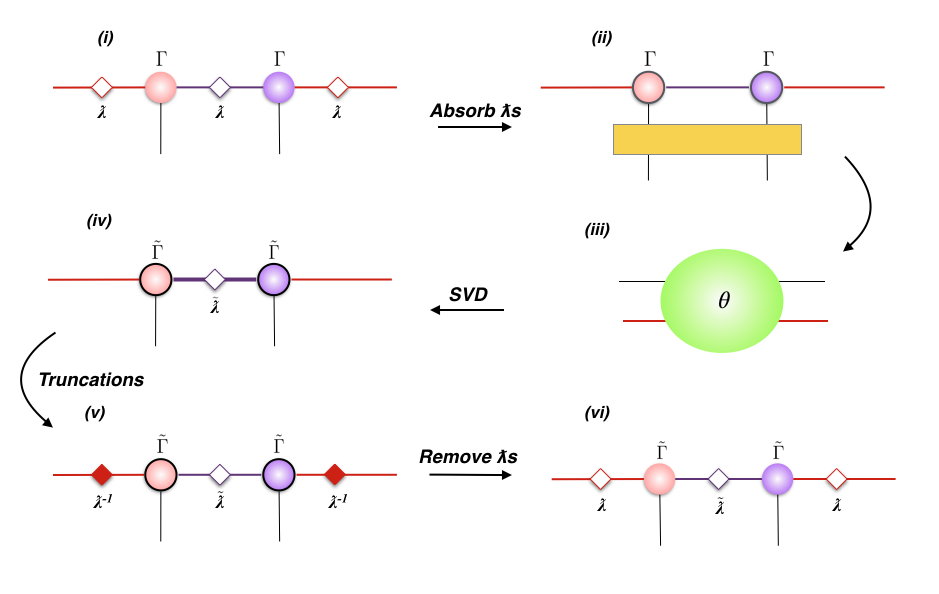
\includegraphics[width=0.90\textwidth]{figures/fig313.png}
	\caption[The tensor network diagrams for the 1-D iTEBD]{ (i)Absorb all $\lambda$ to $\Gamma$. (ii) Contract an evolution operator $e^{-\delta H}$ for evolving the system. (iii) Decompose the tensor $\theta$ by SVD. (iv) Truncate and Update the states and $\lambda$ on the green bond.(v) Remove $
		\lambda$ for obtaining the states. (iv) After updating the states and $\lambda$ on the purple bond, apply the way to update the red bond and repeat all the steps until the ground state convergence.}
	\label{fig314}
\end{figure}

In one dimensional many-body systems, the performance of iTEBD is pretty well. Although the accuracy is little less than DMRG \cite{}, it is still widely applied to study or test models due to its high efficiency.

\subsection{Two-dimensional iTEBD}
\label{2ditebd}

Due to the success in 1-D cases, we desire to extend the framework of iTEBD to simulate 2-D systems . In 2-D systems, we describe the wave functions by the projected entangled pair states (PEPS) rather than MPS. The PEPS structure is an naturally extension of MPS and obey the restriction of MPS. Therefore, it can be expanded to a infinite structure, iPEPS, which are composed by $n$-site translation invariance states. For instance, we can draw an tensor diagram as shown in Fig. \ref{fig315} to represent the wave function of a 2-D many-body system which is composed by 2-site translational symmetric states.

\begin{figure}[ht]
	\centering
	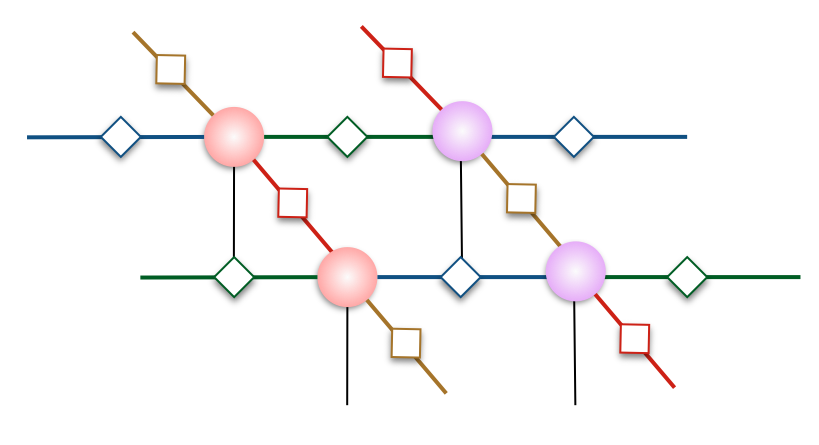
\includegraphics[width=0.6\textwidth]{figures/fig314.png}
	\caption[The tensor diagrams of 2-D lattice]{Four sites unit cell in iPEPS.}
	\label{fig315}
\end{figure}

After building the form of iPEPS, we start to deal with the problem of updating states. The most intuitive method is directional simple update, which means that the states of iPEPS must be updated by iTEBD along four directional moves, namely up, right, down and left. The scheme of implementing 2D-iTEBD is shown as follows which start from right move,

\begin{enumerate}
	\item Initialization: To describe iPEPS states [Fig. \ref{fig316}], we need two random rank-5 tensors $\Gamma^{[A]}_{uldr,\sigma_j}$ and $\Gamma^{[B]}_{uldr, \sigma_j}$ which dimension are $dD^4$, and four random diagonal matrix $\lambda_{u}$, $\lambda_{l}$, $\lambda_{d}$ and $\lambda_{r}$.
	\item Obtain a cluster tensor $\Theta$: As shown in Fig. \ref{fig315}(ii),
		\begin{enumerate}
			\item Absorb the entangled matrices; 
				\begin{align}
					&\Gamma^{\prime [A]}_{uldr,\sigma_i} = \sum_{uldr}{ \lambda_{u}\lambda_{l} \Gamma^{[A]}_{ulrd,\sigma_i} \lambda_{r} \lambda_{d}} \\
					&\Gamma^{\prime [B]}_{uldr,\sigma_j} = \sum_{uld}{\lambda_{d} \Gamma^{B}_{uldr,\sigma_j} \lambda_{u}\lambda_{l}}
				\end{align}
			\item Utilize the evolution operate $U(\tau)$: See Fig. \ref{fig316}(iii)
				\begin{align}
					\Theta = \sum_{r,\sigma_i^{\prime}\sigma_j^{\prime}}{U^{\sigma_i^{\prime}\sigma_j^{\prime}}_{\sigma_i\sigma_j} \Gamma^{\prime\sigma_i [A]}_{uld,r} \Gamma^{\prime \sigma_j[B]}_{r,u^{\prime} l^{\prime} d^{\prime}}}
				\end{align}
				the rank of $\Theta$ is eight and the dimension is $d^2D^6$.
			\end{enumerate}
		\item Decompose $\theta$ into the general form of iPEPS:
		\item Truncation: See Fig. \ref{fig316}(iv), the dimension of bond $r$ increase to $dD^3$. To reduce the consumption, we must truncate the dimension to a smaller $D$.
		\item Absorb the inverse entangled matrix surrounding $\Gamma^{\prime [A]}$ and $\Gamma^{\prime [B]}$: Return to the general form of the iPEPS, as shown in Fig. \ref{fig316}(v).
				\begin{align}
					&\widetilde{\Gamma}^{[A]}_{uldr,\sigma_i} = \sum_{uldr}{ \lambda_{u}^{-1} \lambda_{l}^{-1} \Gamma^{[A]}_{ulrd,\sigma_i} \lambda_{d}^{-1}} \\
					&\widetilde{\Gamma}^{[B]}_{uldr,\sigma_j} = \sum_{uld}{\lambda_{d}^{-1} \Gamma^{[B]}_{uldr,\sigma_j} \lambda_{u}^{-1} \lambda_{l}^{-1}}
				\end{align}
			\item Repeat the steps (2)-(5) to update the others directional moves. To explain more explicitly, the procedures of the up move are shown in Fig. \ref{fig317}.
			\item Iterate the steps (2)-(6) until the wave function converges.
			
In one dimensional many-body systems, the performance of iTEBD is pretty well. Although the accuracy is little less than DMRG \cite{}, it is still widely applied to study or test models due to its high efficiency.

\end{enumerate}

\begin{figure}[ht]
	\centering
	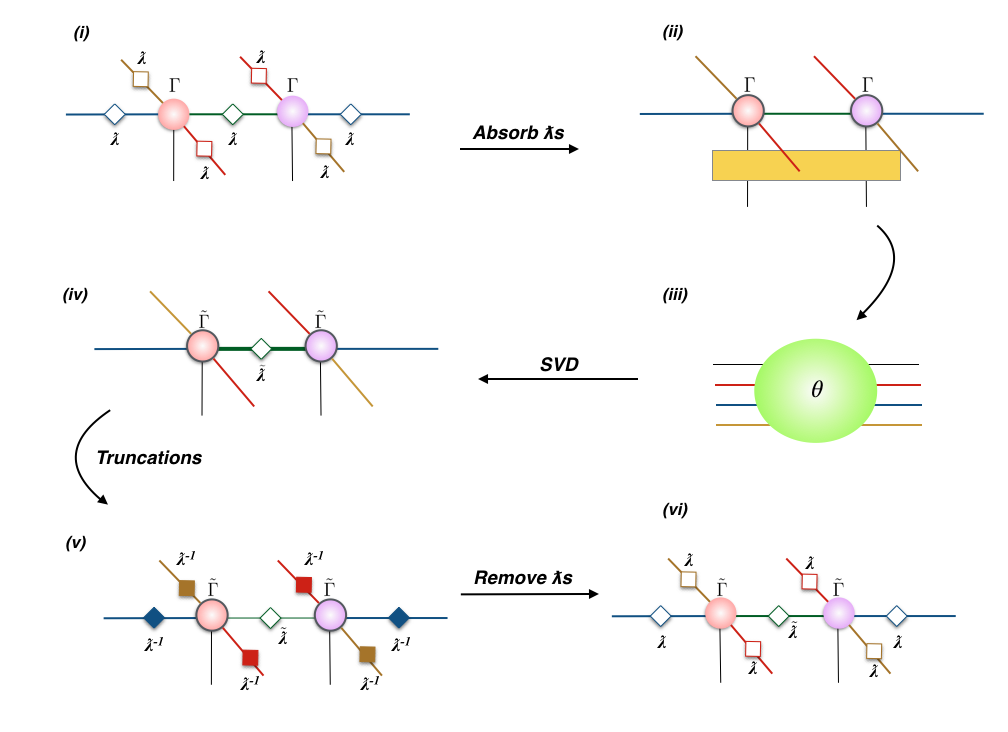
\includegraphics[width=0.80\textwidth]{figures/fig315.png}
	\caption[The tensor network diagrams of updating the green bond in iPEPS with 2D-iTEBD]{Absorb all $\lambda$ to $\Gamma$. (ii) Contract an evolution operator $e^{-\delta H}$ for evolving the system. (iii) Decompose the tensor $\theta$ by SVD. (iv) Truncate and Update the states and $\lambda$ on the green bond.(v) Remove $\lambda$ for obtaining the states. (iv) Obtain a original form of iPEPS. Repeat all the step to update the other bonds until the ground state energy convergence}
	\label{fig316}
\end{figure}

	\begin{figure}[ht]
	\centering
	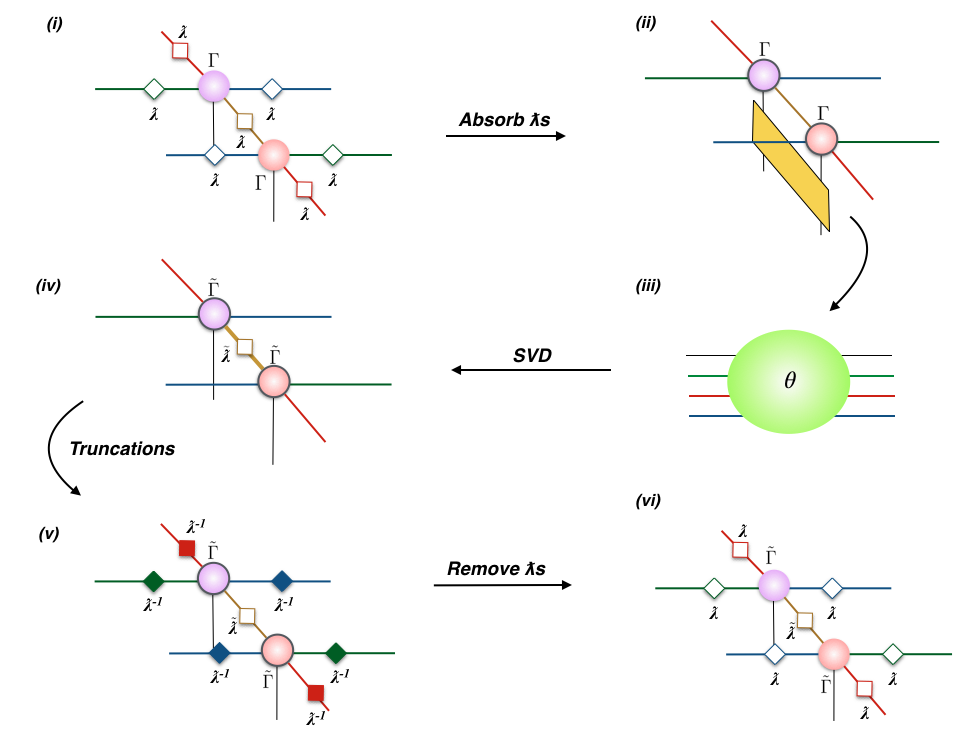
\includegraphics[width=0.80\textwidth]{figures/fig316.png}
	\caption[The tensor network diagrams of updating the yellow bond in iPEPS with 2D-iTEBD]{Update the yellow bond and the steps are similar to Fig.\ref{fig315}}
	\label{fig317}
	\end{figure}

\section{Ameliorate two-dimensional iTEBD}
\label{2dhastin}

The directional simple update discussed in section.\ref{2ditebd} can obtain good iPEPS states in toy models. However, in some complicated models it becomes unstable and inefficient. The reason is that there are too many multiplications of pseudo-inverse $\lambda^{-1}$ at the step Fig.\ref{fig316}(v). In numerical methods, it's dangerous to divide a value which is equal or approach to zero. In other words, the more inverse operations, the more probability of destroying algorithms and harder to converge. Hence, \textit{M. B. Hastings} develop another scheme to improve that problem \cite{hastings_light-cone_2009}. The procedures from the right is shown as follows,
%#############
\begin{enumerate}
	\item Initialization: As directional simple update, we declare two random $\Gamma^{[A]}$ and $\Gamma^{[B]}$, and four random diagonal matrix $\lambda_{u}$, $\lambda_{r}$, $\lambda_{l}$ and $\lambda_{d}$ to describe the wave function. \ref{fig318}(i). However, the definition of $\Gamma^{[A]}$ and $\Gamma^{[B]}$ are different. In this scheme,
		\begin{align}
			\Gamma^{[A]}_{ulrd,\sigma_i} \equiv \sum_{ur}{\lambda_{u} \Gamma^{[A_s]}_{ulrd,\sigma_i} \lambda_{r}} \\
			\Gamma^{[B]}_{ulrd,\sigma_j} \equiv \sum_{dl}{\lambda_{d} \Gamma^{[B_s]}_{ulrd,\sigma_j} \lambda_{l}}
		\end{align}
		where $\Gamma^{[A_s]}_{ulrd,\sigma_i}$ and $\Gamma^{[B_s]}_{ulrd,\sigma_j}$ are the definition in directional simple update. [In sec.\ref{2ditebd}].
	\item Obtain the cluster tensor $C$: As shown in Fig. \ref{fig318}(b),
			\begin{enumerate}
				\item Absorb the entangled matrices $\lambda_{u}$ into  $\Gamma^{[B]}_{ulrd,\sigma_j}$:
					\begin{align}
						%&\Gamma^{\prime [A]}_{uldr, \sigma_j} = \sum_{dl}{\lambda_{i} \Gamma^{A}_{ij \sigma_i} \lambda_{j}} \\
						&\Gamma^{\prime [B]}_{uldr, \sigma_j} = \sum_{u}{\Gamma^{[B]}_{uldr,\sigma_j} \lambda_{u}}
					\end{align}
				\item Contract the tensors $\Gamma^{[A]}$, $\Gamma^{\prime [B]}$ and the evolution operate $U(\tau)$: 
					\begin{align}
						C = \sum_{r,\sigma_i^{\prime}\sigma_j^{\prime}}{U^{\sigma_i^{\prime}\sigma_j^{\prime}}_{\sigma_i\sigma_j} \Gamma^{\sigma_i [A]}_{uld,r} \Gamma^{\prime \sigma_j[B]}_{r,u^{\prime} l^{\prime} d^{\prime}}}
					\end{align}
			\end{enumerate}
		\item Obtain the cluster tensor $\Theta$: In the step, the entanglement surrounding $\Gamma^{[A]}$ would be absorbed in the tensor $C$,
			\begin{align}
				\Theta = \sum_{dl}{\lambda_{d} \lambda_{l} C^{udl,\sigma_i}_{u^{\prime}d^{\prime}l^{\prime},\sigma_j}}
			\end{align}
		\item Decompose $\theta$ into the general form of the iPEPS and truncate the updated bond: This step is same as directional simple update, see Fig. \ref{fig318}(v)
		\item Update $\Gamma^{[A]}$: Due to the tensor $C$ does not contain the entanglement surrounding $\Gamma^{[A]}$, the updated $\Gamma^{[A]}$ can be obtained by contracting tensors $C$ and $\widetilde{\Gamma}^{[B]}$
			\begin{align}
				\Gamma^{[A]} = \sum_{u^{\prime}l^{\prime}r^{\prime}\sigma_j}{C^{udl,\sigma_i}_{u^{\prime}d^{\prime}l^{\prime},\sigma_j} \widetilde{\Gamma}^{\sigma_j [B]}_{u^{\prime}d^{\prime}l^{\prime}}}
			\end{align}
		\item Absorb the inverse $\lambda_{u}$ into $\widetilde{\Gamma}^{[B]}_{ulrd,\sigma_j}$:
			\begin{align}
				\Gamma^{[B]} = \sum_{u}{\lambda_{u}^{-1}\widetilde{\Gamma}^{[B]}_{ulrd,\sigma_j}}
			\end{align}
			, which is shown as Fig. \ref{fig318}.
		\item Repeat the steps (2)-(5) to update the others directional moves, down, left, up.  
		\item Iterate the steps (2)-(6) until the wave function converges.
\end{enumerate}

In the procedures of directional simple update, there are six pseudo-inverse $\lambda^{-1}$ must be absorbed in each iteration. Relatively, in this scheme we just need multiply an pseudo-inverse $\lambda^{-1}$ in step(6). Nevertheless, the consumption of updating states in step(5) is higher than the update step in directional simple update and cost more time in each iteration. The stability is able to make the wave function converge in less iterations.

\begin{figure}[ht]
	\centering
	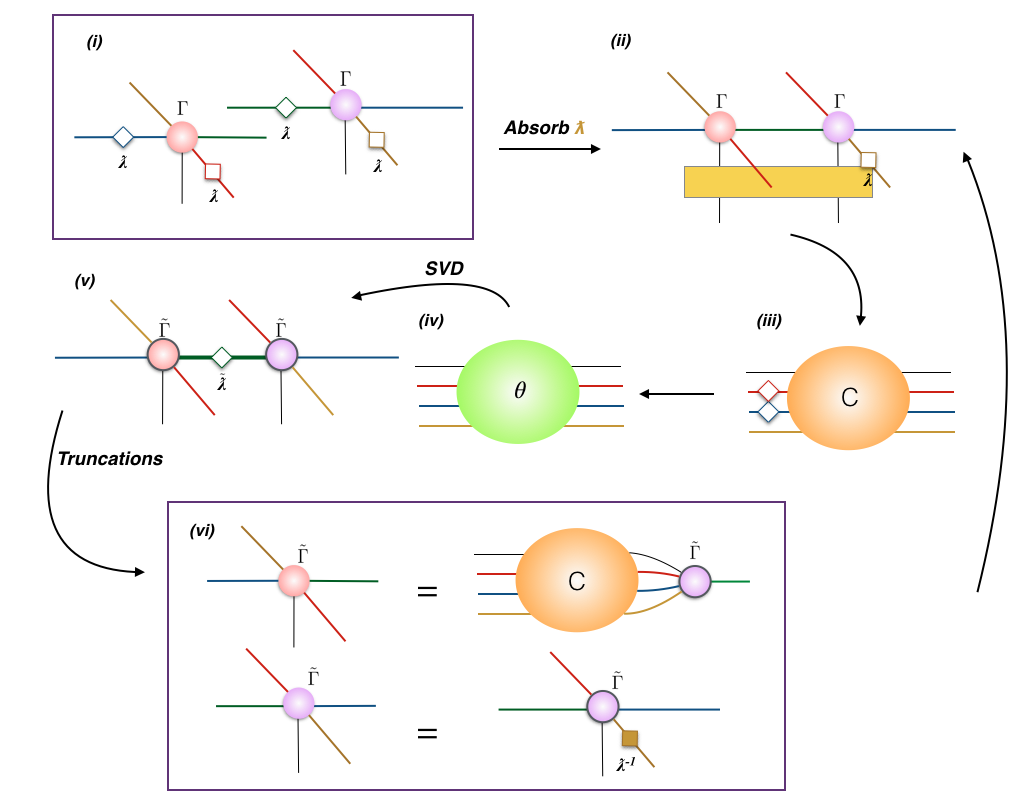
\includegraphics[width=1.00\textwidth]{figures/fig317.png}
	\caption[The tensor network diagrams for the 2-D iTEBD with QR decomposition]{The tensor network diagrams for the ameliorated 2-D iTEBD.}
	\label{fig318}
\end{figure}

\section{Optimizations}
\label{2dopt}
\subsection{Initialization}
\label{2doptInit}
\begin{figure}[ht]
	\centering
	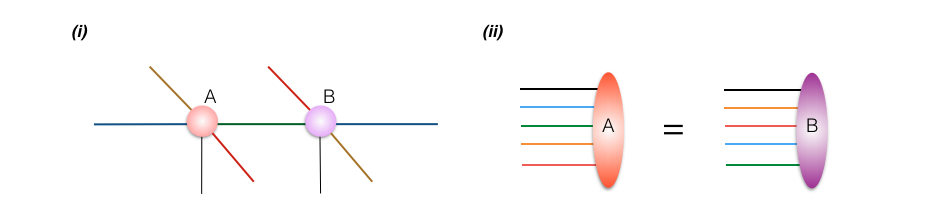
\includegraphics[width=1.00\textwidth]{figures/fig321.png}
	\caption[The diagrams of initializing projected entangled pair states]{(i) The structure of PEPS, (ii) The initialization of states}
	\label{fig321}
\end{figure}

Intuitively, the initialization of states should not affect the result. However, it's a serious misunderstanding. Actually, stating from a awful initial sates may break the algorithms or hardly converge.

From the viewpoint of physics, translational invariance is one of essential properties in many-body system, So we can assume that the group state on two sites should be similar. For instance, if the TN diagram of the states is shown as Fig \ref{fig321}(i), Fig \ref{fig321}(ii) might be the better way to initialize the states.

\subsection{QR and LQ decomposition}
\label{2doptQR} 
In the section \ref{2ditebd} and \ref{2dhastin}, we have introduced to two different methods to implement 2D-iTEBD. However, it is hard to apply them to study when the dimension of the virtual bonds become larger because of the rapid increment of the dimension of tensor $\Theta$ [Fig. \ref{fig316}(iii) and Fig. \ref{fig318}(iii)] which is a rank-8 tensor with dimension $d^2D^6$. In addition to the problem of their consumption, the singular value decomposition, which time complexity proportional $O(NM^2)$, is expensive.  Therefore, in this section we apply QR and LQ decomposition to reduce the rank of $\Theta$.

The QR decomposition allows to decompose a real or complex matrix $A_{m,n}$, with $m \geq n$, into a $m \times m$ unitary matrix $Q$ and a $m \times n$ upper triangular matrix $R$. However, in bottom $(m-n)$ rows of $R$ are filled with zeros. Hence, matrix $Q$ and $R$ can be truncated,
\begin{align}
	A = QR = Q \begin{bmatrix} R_1 \\ 0 \end{bmatrix} = \begin{bmatrix} Q_1, Q_2 \end{bmatrix} \begin{bmatrix} R_1 \\ 0 \end{bmatrix} = Q_1 R_1, 
\end{align}
where $Q_1$ is a $(m \times n)$ unitary matrix and $R_1$ is a $(n \times n)$ upper triangular matrix. Analogously, the LQ decomposition can decompose a matrix $A_{m,n}$, with $m \leq m$ into a $m \times n$ lower triangular matrix $L_1$ and a $m \times n$ unitary matrix $Q_1$, 
\begin{align}
	A = LQ = \begin{bmatrix} L_1, 0 \end{bmatrix} Q = \begin{bmatrix}  L_1, 0\end{bmatrix} \begin{bmatrix} Q_1 \\ Q_2 \end{bmatrix} = L_1 Q_1, 
\end{align}

In the case of directional simple update, most of the steps of implementing with QR decomposition is similar to original one, see Fig. \ref{fig318}. There are just two differences, 
\begin{enumerate}
	\item After the entangled matrices $\lambda$s are absorbed, we decompose the states $\Gamma^{[A]}$ into a unitary matrix $X$ and a upper triangular matrix $a_R$,
		\begin{align}
			\Gamma^{[A]}_{\chi_d \chi_l \chi_u, \chi_{\sigma_i} \chi_r} = X_{\chi_d \chi_l \chi_u, \chi_{\sigma_i} \chi_r} {a_R}_{\chi_{\sigma_i} \chi_r,\chi_{\sigma_i} \chi_r}
		\end{align}
		and decompose $\Gamma^{[A]}$ into a unitary matrix $Y$ and a lower triangular matrix $b_L$
		\begin{align}
			\Gamma^{[B]}_{\chi_{\sigma_j} \chi_r, \chi_d \chi_l \chi_u} = {b_L}_{\chi_{\sigma_j} \chi_r,\chi_{\sigma_j} \chi_r} Y_{\chi_{\sigma_i} \chi_r, \chi_d \chi_l \chi_u} 
		\end{align}
		where $\chi_n$ means the dimension of the bond $n$. See Fig. \ref{fig318}(ii).
	\item Contract $X$ and $a_R$ into $\Gamma^{[A]}$ and $b_L$ and $Y$ into $\Gamma^{[B]}$ before the inverse matrices are absorbed. See Fig. \ref{fig318}(v).

\end{enumerate}
\begin{figure}[H] 
	\centering 
	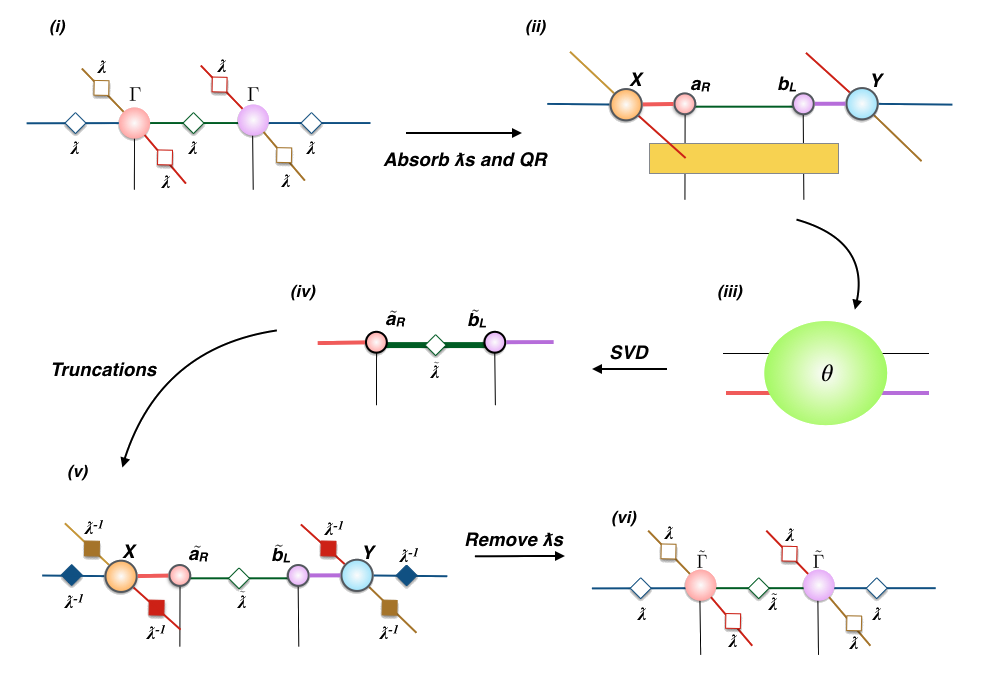
\includegraphics[width=1.00\textwidth]{figures/fig318.png} 
	\caption[The tensor network diagrams for the ameliorated 2-D iTEBD with QR decompositiont]{The tensor network diagrams for the ameliorated 2-D iTEBD.} 
	\label{fig318} 
\end{figure} 

\begin{figure}[!ht]
	\centering
	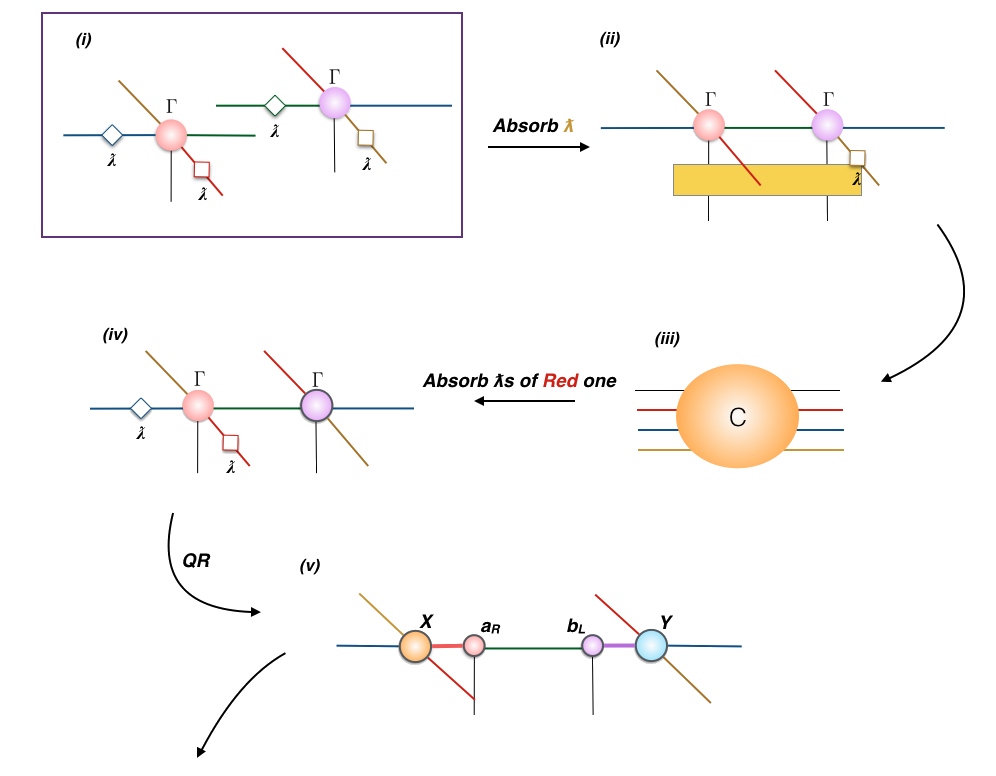
\includegraphics[width=1.00\textwidth]{figures/fig319.png}
	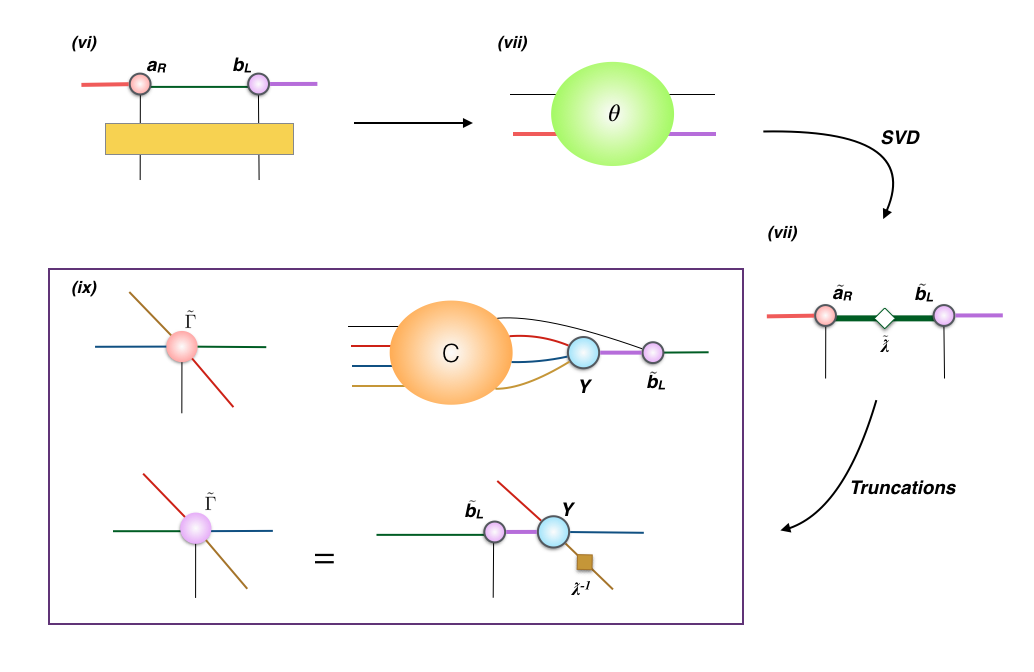
\includegraphics[width=1.00\textwidth]{figures/fig320.png}
	\caption[The tensor network diagrams for the ameliorated 2-D iTEBD with QR decompositiont]{The tensor network diagrams for the ameliorated 2-D iTEBD.}
	\label{fig319}
\end{figure}

Nevertheless, the main idea to reduce the tensor $\Theta$ in ameliorate 2D-iTEBD is same as in directional simple update. The scheme becomes more complicated, see Fig. \ref{fig318}, 

\begin{enumerate}
	\item Instead absorb $\lambda_d$ and $\lambda_l$ into the cluster tensor $C$, we absorb them into $\Gamma^{[A]}$
		\begin{align}
			\Gamma^{\prime [A]}_{uldr,\sigma_i} = \sum_{dl}{\lambda_l \Gamma^{[A]}_{uldr,\sigma_i} \lambda_d}
		\end{align}
		and apply the QR and LQ decomposition to split $\Gamma^{\prime [A]}$ and $\Gamma^{\prime [B]}$ into $X\cdot a_R$ and $b_L \cdot Y$. see Fig. \ref{fig319}(iv) and Fig. \ref{fig319}(v) 
	\item Obtain $\widetilde{\Gamma}^{[A]}$ by contracting tensor $C$, $Y$ and $\b_L$, as shown in Fig. \ref{fig319}(ix)
		\begin{align}
			\widetilde{\Gamma}^{[A]}_{urld, \sigma_i} = \sum_{u^{\prime}l^{\prime}d^{\prime}\sigma_j,q}{C^{dlu\sigma_i}_{d^{\prime}l^{\prime}u^{\prime}\sigma_i}Y_{d^{\prime}l^{\prime}u^{\prime}q}{b_L}_{qr}}
		\end{align}
		and obtain $\widetilde{\Gamma}^{[B]}$ by contracting $Y$, $b_L$ and $\lambda_u^{-1}$
		\begin{align}
			\widetilde{\Gamma}^{[B]}_{urld,\sigma_j} = sum_{q}{{b_L}_{rq}Y_{uld\sigma_j q}\lambda_u^{-1}}
		\end{align}
\end{enumerate}

Through these changed, the tensor $\Theta$ is reduced to and rank-4 tensor, with dimension $d^2D^2$.

\subsection{Truncation Error}
In order to avoid the dimension of the virtual bonds increase exponentially, after decomposing the tensor $\Theta$, we will truncate the updated bond from $dD^3$ or $d^2D$ to $D$. However, if the singular values are not concentrated to the leading elements, some influential features and basis would be dropped and the algorithms might be broken. Therefor, we set a truncate error $\varepsilon$, 
\begin{align}
	\varepsilon = 
\end{align}
to determinate the number of basis should be remained.

\section{Comparison}

So far, we have benchmarked the improved iTEBD. 

\label{Comparison}
\subsection{Different Initializations}

\begin{figure}[ht]
	\centering
	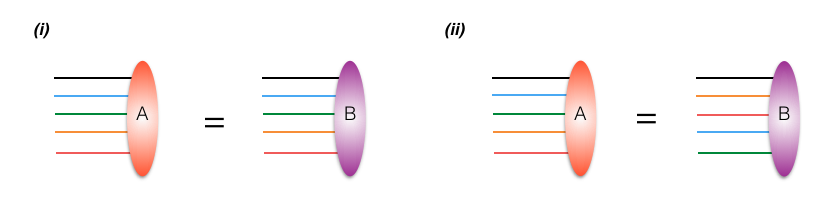
\includegraphics[width=1.00\textwidth]{figures/fig322.png}
	\caption[Different methods to initialize the states]{(i) Type 1, (ii) Type 2}
	\label{fig322}
\end{figure}

See Fig \ref{fig323}, the both cases are 

\begin{figure}[ht]
	\centering
	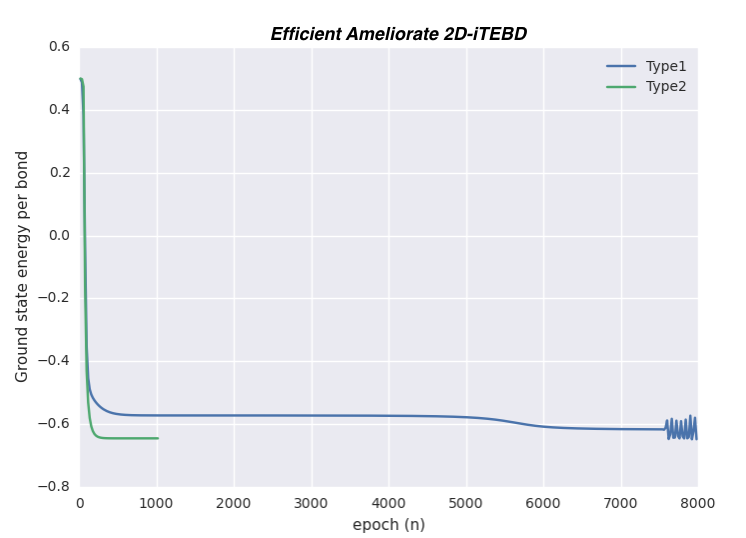
\includegraphics[width=0.75\textwidth]{figures/fig323.png}
	\caption[Comparison the results of Heisenberg model on square lattice which are obtaining from different initial states.]{The Blue line represents updating tensors from the initial state shown in Fig \ref{fig322} (i) and the green one represents updating from Fig \ref{fig322} (ii)}
	\label{fig323}
\end{figure}

\begin{figure}[ht]
	\centering
	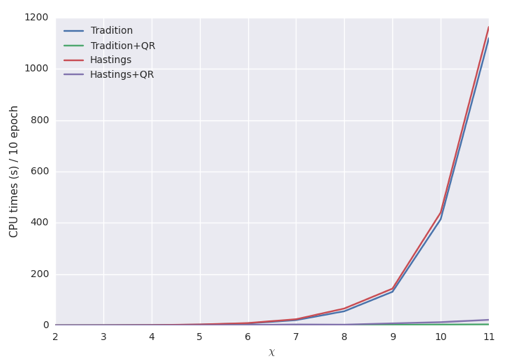
\includegraphics[width=0.75\textwidth]{figures/fig324.png}
	\caption[CPU times of different 2D-iTEBD with fixed trucation error]{}
	\label{fig324}
\end{figure}

\begin{figure}[ht]
	\centering
	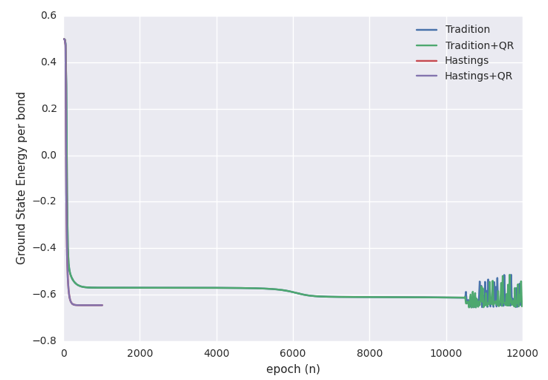
\includegraphics[width=0.75\textwidth]{figures/fig325.png}
	\caption[Per epoch energy of Heisenberg model on 2d square lattice with fixed truncation error]{}
	\label{fig325}
\end{figure}

\begin{figure}[ht]
	\centering
	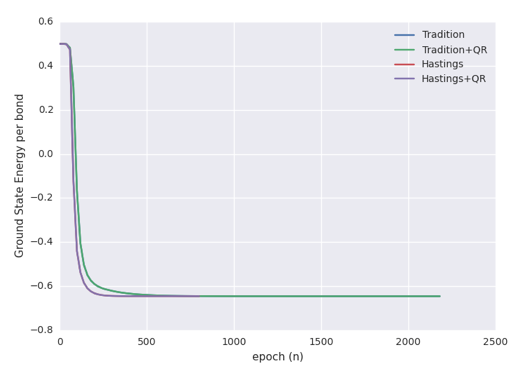
\includegraphics[width=0.75\textwidth]{figures/fig326.png}
	\caption[CPU times of different 2D-iTEBD with dynamic trucation error]{}
	\label{fig326}
\end{figure}

\begin{figure}[ht]
	\centering
	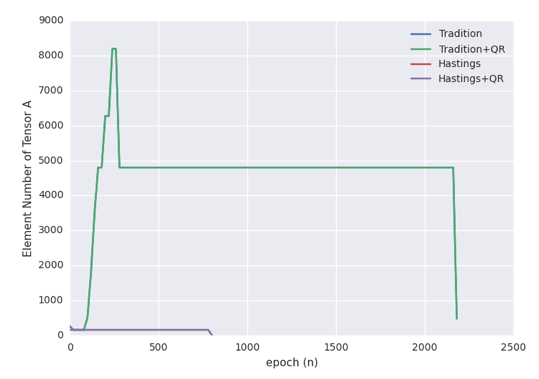
\includegraphics[width=0.75\textwidth]{figures/fig327.png}
	\caption[Per epoch energy of Heisenberg model on 2d square lattice with dynamic truncation error]{}
	\label{fig327}
\end{figure}
